\makeatletter\let\ifGm@compatii\relax\makeatother
\documentclass[mathserif,fleqn]{beamer}

\mode<presentation>
{
  %\usetheme{Warsaw}
  \usetheme{Antibes}
  %\usetheme{Boadilla}
  \setbeamercovered{transparent}
}
%\usepackage{beamerthemesplit}
\usepackage{beamerthemeshadow}
%\usepackage[width=2cm,dark,tab]{beamerthemesidebar}

\usepackage{pgf,pgfarrows,pgfnodes,pgfautomata,pgfheaps}
%\usepackage[tbtags]{amsmath}
\usepackage{amsmath,amssymb,amsfonts}
\usepackage{color,xcolor}
\usepackage{graphicx}
\usepackage{multimedia}
\usepackage{manfnt}
\usepackage[english]{babel}
\usepackage{algorithmic}
\usepackage{algorithm}
\usepackage{setspace}
\usepackage[timeinterval=1]{tdclock}
\usepackage{tikz}
\usetikzlibrary{shapes,arrows}
%\beamersetaveragebackground{black!10}
\usefonttheme[stillsansseriflarge]{serif}
\usepackage{times}
\beamertemplatesolidbackgroundcolor{white}
%\beamertemplateshadingbackground{white!90}{structure!1}
%\beamertemplatesolidbackgroundcolor{white!90!blue}
\beamertemplatetransparentcovereddynamic
\beamertemplateballitem
\beamertemplatenumberedballsectiontoc
%\beamertemplatelargetitlepage
\beamertemplateboldpartpage
\setbeamertemplate{itemize item}[triangle]
%\setbeamertemplate{footline}[page number]
\setbeamertemplate{footline}[text line]{%
\llap{Songpeng Zu\hspace{-5mm}}\centerline{\strut MulTQSAR}\llap{\insertframenumber\hspace{-5mm}}}
\newtheorem{jiashe}{Assumption~}[section]


%\setbeamertemplate{item}[triangle]
\graphicspath{{./figures/}}
%\AtBeginSection[]{
%  \frame<handout:0>{
%    \frametitle{Content}
%    \tableofcontents[current,currentsubsection]
%  }
%}
%\AtBeginSubsection[]{
%  \frame<handout:0>{
%    \frametitle{Content}
%    \tableofcontents[current,currentsubsection]
%  }
%}
% Table rules
\def\toprule{\noalign{\ifnum0=`}\fi\hrule \@height 0.5pt \hrule \@height 6pt \@width 0pt \futurelet
   \@tempa\@xhline}
\def\midrule{\noalign{\ifnum0=`}\fi \hrule \@height 6.75pt \@width 0pt \hrule \@height 0.5pt
    \hrule \@height 6pt \@width 0pt \xfuturelet \@tempa\@xhline}
\def\botrule{\noalign{\ifnum0=`}\fi \hrule \@height 5.75pt \@width 0pt \hrule \@height 0.5pt \futurelet
   \@tempa\@xhline}

% Define block styles
\tikzstyle{decision} = [diamond, draw, fill=blue!20,
    text width=4.5em, text badly centered, node distance=2.5cm, inner sep=0pt]
\tikzstyle{block} = [rectangle, draw, fill=blue!20,
    text width=5em, text centered, rounded corners, minimum height=4em]
\tikzstyle{line} = [draw, -latex']
\tikzstyle{cloud} = [draw, ellipse,fill=red!20, node distance=2.5cm,
    minimum height=2em]


\begin{document}

\title{Qualitatively Predicting Compound-Protein Interactions by Multi-Task Learning}
\author[zusp]{PhD Candidate: Songpeng Zu\\Advisor: Prof.\ Shao Li}
\institute[tnlist]{
  Bioinformatics Lab, Department of Automation \\Tsinghua university
}
%\date[\initclock\mmddyyyy\tddate\ \ \hhmmss\tdtime]{\today}
\date[\initclock\tdtime]{\today}
%\maketitle
\frame[plain]{\titlepage}

\section*{outline}
\frame{
    \setbeamercolor{uppercol}{fg=white,bg=teal}
    %\setbeamercolor{lowercol}{fg=black,bg=lime}
    \begin{beamerboxesrounded}[upper=uppercol,shadow=true]{outline}
      \begin{spacing}{1.2}
        \begin{itemize}
        \item
          Background:
          \begin{itemize}
          \item Quantitative Structure-Activity Relationship (QSAR)
          \item Multi-task Learning
          \end{itemize}
        \item
          Method: hierarchical Bayesian model called MulTQSAR
        \item
          Result: reduce MSE on PeptideGPCR
        \item
          Discussion:
          \begin{itemize}
          \item Sparsity and feature selection
          \item Multi-task Deep learning on QSAR
          \end{itemize}
        \end{itemize}
      \end{spacing}
    \end{beamerboxesrounded}
}
\section{Background}
\subsection{Quantitative Structure-Activity Relationship}
\frame{
\frametitle{Compound-Protein Interactions (CPIs)}
%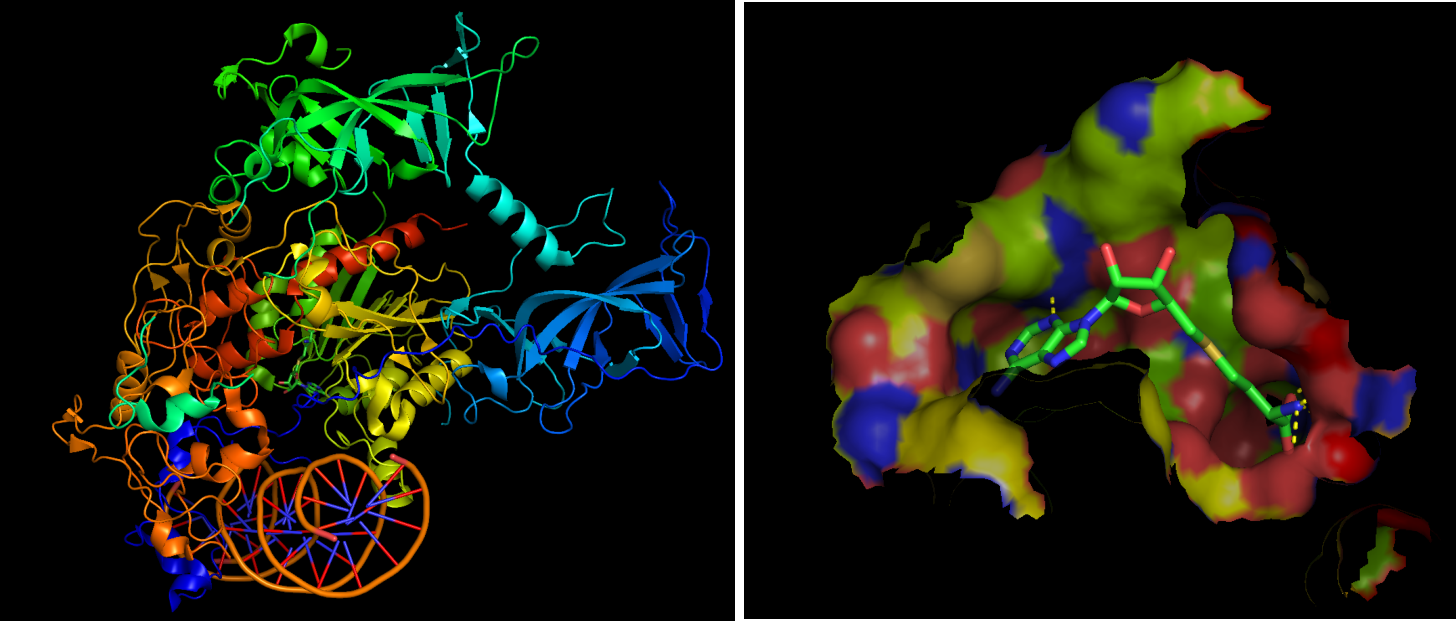
\includegraphics[width=\textwidth]{one-protein-one-drug}
}
\frame{
\frametitle{Protein Versus Multiple Compounds}
% 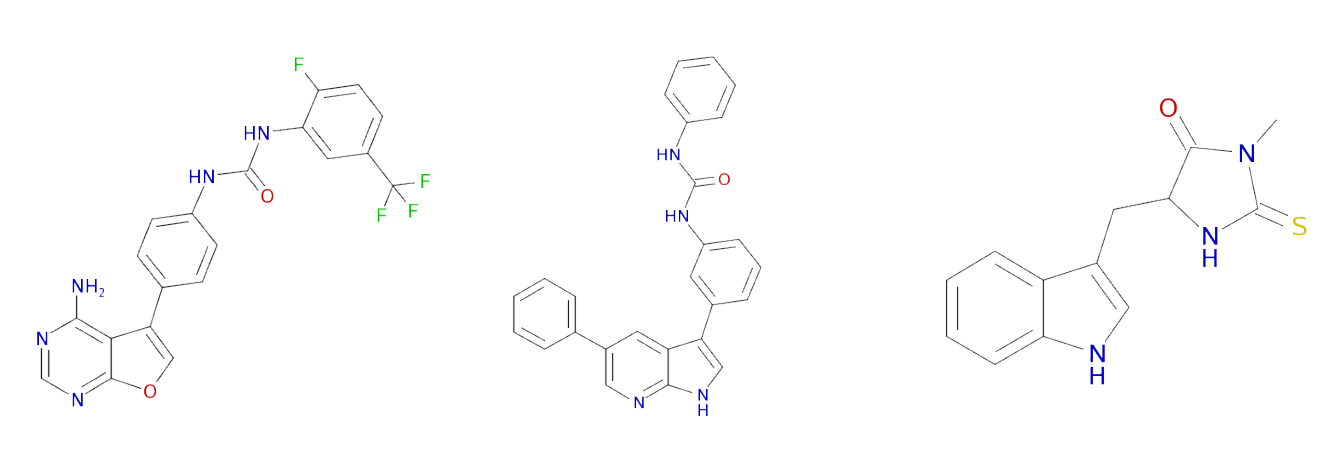
\includegraphics[width=\textwidth]{one-protein-multi-drugs}
}
\frame{
\frametitle{Chemical Space: Representation of Compounds}
% \includegraphics[width=\textwidth]{compound-representation}
}
\frame{
\frametitle{Single Protein QSAR Model}
For the protein $l$, we have $n_{l}$ compounds. Let $\mathbf{x}_{i}^{l}$
represents the compound $i$'s features in the chemical space, and
$\mathbf{y}_{i}^{l}$ represents the interaction affinity between the compound
$i$ and protein $l$. \\QSAR is then to solve the problem:
\begin{equation}
f = \arg\min_{f}\mathcal{L}\left(\mathbf{y}^{l},f(\mathbf{X}^{l})\right)
\end{equation}
in which, $\mathbf{X}^{l}={(\mathbf{x}_{1}^{l},\cdots,\mathbf{x}_{n_{l}}^{l})}^{t}$,
$\mathcal{L}(~,~)$ is the loss function. Usually we treat is as a linear
regression model, $\mathit{i.e.}$,
\begin{equation}
\mathbf{\omega}^{l} = \arg\min_{\mathbf{\omega}^{l}}{\lVert
  \mathbf{y}^{l}-\mathbf{X}^{l}\mathbf{\omega}^{l} \rVert}^{2}
\end{equation}
}
\frame{
\frametitle{Protein Family}
% \includegraphics[width=\textwidth]{protein-family-multisequence}
}
\frame{
\frametitle{Can We Learn QSAR Models In A Protein Family ?}
% 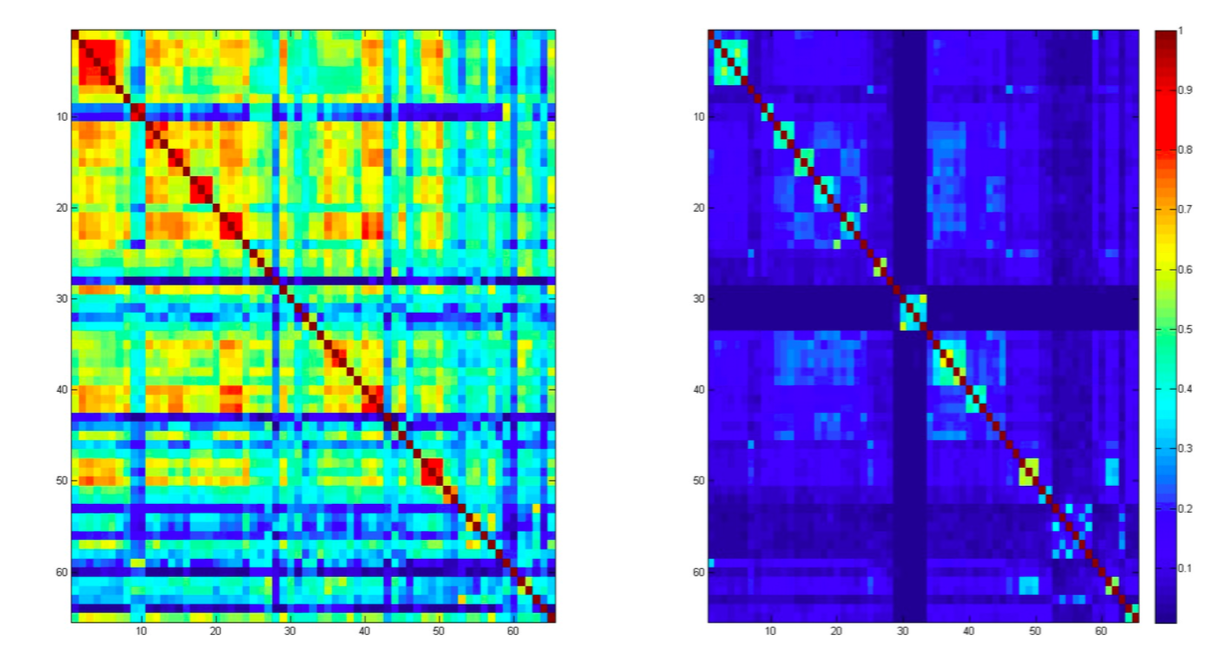
\includegraphics[with=\textwidth]{GPCR-seq-compounds}
}
\subsection{Multi-task Learning}
\frame{
\frametitle{Learning Different But Similar Tasks}
\begin{itemize}
\item Learning multiple tasks together, one type of transfer learning (Pan
  S. and Yang Q., 2010).
\item Examples:
\begin{enumerate}
\item Multi-task feature selection (Obozinski G., Taskar B., Jordan, M., 2006)
\begin{equation}
\min_{\omega}\sum_{l=1}^{L}\frac{1}{N_{l}}\sum_{i=1}^{N_{l}}\mathcal{L}(\omega^{l},x_{i}^{l},y_{i}^{l})
+ \lambda\sum_{j=1}^{p}{\lVert \omega_{j}\rVert}^{2}
\end{equation}
in which, $p$ is the feature number, $L$ is the task number.
\item Adaptive multi-task LASSO (Lee S., Zhu J., and Xing E., 2010)
\begin{equation}
\min_{\omega}\frac{1}{2}\sum_{l=1}^{L}{\lVert Y^{l} - X\omega^{l}\rVert}_{2}^{2} +
\lambda_{1}\sum_{j=1}^{p}\theta_{j}\sum_{l=1}^{L}|\omega_{j}^{l}| + \lambda_{2}\sum_{j=1}^{p}\rho_{j}{\lVert \omega_{j} \rVert}_{2}
\end{equation}
\end{enumerate}
\end{itemize}
}
\section{Method}
\subsection{Mathematical formulation}
\frame{
\frametitle{Hierarchical Bayesian Model}
Suppose $ \mathbf{\mathcal{D}}_{j} = \left\{\textbf{X}_{j},\textbf{y}_{j}\right\},j=1,...,m$, and $\textbf{X}_{j}\in\mathbb{R}^{d\times n_{j}}$. Then we have
\begin{equation}
  \mathbf{y}_{j} \sim \mathcal{N}\left(\mathbf{X}_{j}^{T}\mathbf{\omega}_{j},\sigma_{y}^{2}\mathbf{I}\right)
\end{equation}
Since different groups data may share similar features, we assume $\mathbf{\omega}_{j}$ have the same mean on the prior distribution.
\begin{equation}
  \mathbf{\omega}_{j} \sim \mathcal{N} \left(\mathbf{\omega}_{\ast},\sigma_{j}^{2}\mathbf{I}\right)
\end{equation}
In which,
\begin{equation}
  \mathbf{\omega}_{\ast} \sim \mathcal{N} \left(\mathbf{\mu},\mathbf{\sigma}_{\ast}^2\mathbf{I}\right)
\end{equation}
}
\subsection{Loglikehood Function}
\frame{
Suppose, for simplicity, that $\mathbf{\mu}=\textbf{0}$, $p(\sigma_{y}^2)\propto 1$, and that $\sigma_{j}^2$ and $\sigma_{\ast}$ are fixed. Let
$\Theta = \left\{\mathbf{\omega}_j, j=1,...,m,\mathbf{\omega}_\ast,\sigma_{y}^2\right\}$. We have
\begin{equation}
\small
\begin{aligned}
  &\mathcal{L}_{hier}(\mathcal{D};\Theta) =
  \mathcal{L}_{orig}(\mathcal{D}| \Theta)+ \textit{logp}(\Theta)\\
  &=\sum_{j}\left(\textit{logp}(\mathcal{D}_{j}|\mathbf{\omega}_{j})-\frac{\parallel\mathbf{\omega}_{j}-\mathbf{\omega}_{\ast}\parallel^{2}}{2\sigma_{j}^2}\right)
  -\frac{\parallel\mathbf{\omega}_{\ast}\parallel^{2}}{2\sigma_{\ast}^2}\\
  &- \overbrace{\sum_{j}\frac{d}{2}\textit{log}(2\pi\sigma_{j}^2)-\frac{d}{2}\textit{log}(2\pi\sigma_{\ast}^2)}^{\textit{Const}}\\
  &=\sum_{j}\left(-\frac{\parallel\mathbf{y}_{j}-\mathbf{X}^{T}_{j}\mathbf{\omega}_{j}\parallel^{2}}{2\sigma_{y}^2}-\frac{\parallel\mathbf{\omega}_{j}-\mathbf{\omega}_{\ast}\parallel^{2}}{2\sigma_{j}^2}\right)-
  \frac{\parallel\mathbf{\omega}_{\ast}\parallel^{2}}{2\sigma_{\ast}^2}-\sum_{j}\frac{n_{j}}{2}\textit{log}(2\pi\sigma_{y}^2)\\
  &- \overbrace{\sum_{j}\frac{d}{2}\textit{log}(2\pi\sigma_{j}^2)-\frac{d}{2}\textit{log}(2\pi\sigma_{\ast}^2)}^{\textit{Const}}
\end{aligned}
\end{equation}
}
\subsection{Optimization: L-BFGS-B}
\frame{
L-BFGS-B optimization method is then used following the gradient below.
\begin{equation}
\small
\begin{aligned}
  \frac{\partial\mathcal{L}_{hier}(\mathcal{D};\Theta)}{\partial\mathbf{\omega}_j}
  &= -\frac{1}{2\sigma_{y}^2}\frac{\parallel\mathbf{y}_j-\mathbf{X}_{j}^{T}\mathbf{\omega}_j\parallel^2}{\partial\mathbf{\omega}_j}
  -\frac{1}{2\sigma_{j}^2}\frac{\parallel\mathbf{\omega}_j-\mathbf{\omega}_{\ast}\parallel^{2}}{\partial\mathbf{\omega}_j}\\
  &=\frac{\mathbf{X}_j\mathbf{y}_j}{\sigma_{y}^2}+\frac{\mathbf{\omega}_{\ast}}{\sigma^2_j}-
  \left(\frac{\mathbf{X}_j\mathbf{X}_j^{T}}{\sigma_{y}^2}+\frac{1}{\sigma_{j}^2}\mathbf{I}\right)\mathbf{\omega}_{j}
\end{aligned}
\end{equation}
\begin{equation}
\small
  \frac{\partial\mathcal{L}_{hier}(\mathcal{D};\Theta)}{\partial\mathbf{\omega}_{\ast}}
  =-\sum_j\frac{\mathbf{\omega}_{\ast}-\mathbf{\omega}_j}{\sigma_{j}^2}-\frac{\mathbf{\omega}_{\ast}}{\sigma_{\ast}^2}
\end{equation}
\begin{equation}
\small
  \frac{\partial\mathcal{L}_{hier}(\mathcal{D};\Theta)}{\partial\sigma_{y}^2}
  =\frac{\sum_j\parallel\mathbf{y}_j-\mathbf{X}_{j}^{T}\mathbf{\omega}_j\parallel^2}{2(\sigma_{y}^2)^2}-\frac{n}{2\sigma_{y}^2}
\end{equation}
where n is the total number of samples in all the groups.
}
\subsection{Data Sets}
\frame{
%\frametitle{Data Sets}
\begin{itemize}
  \item 210,000 CPIs including more than 1,000 proteins from 20 protein families, and  150,000 compounds.
  \item 22 physicochemical properties and 881 chemical substructures as the compounds' features.
\end{itemize}
\begin{figure}
  \centering
  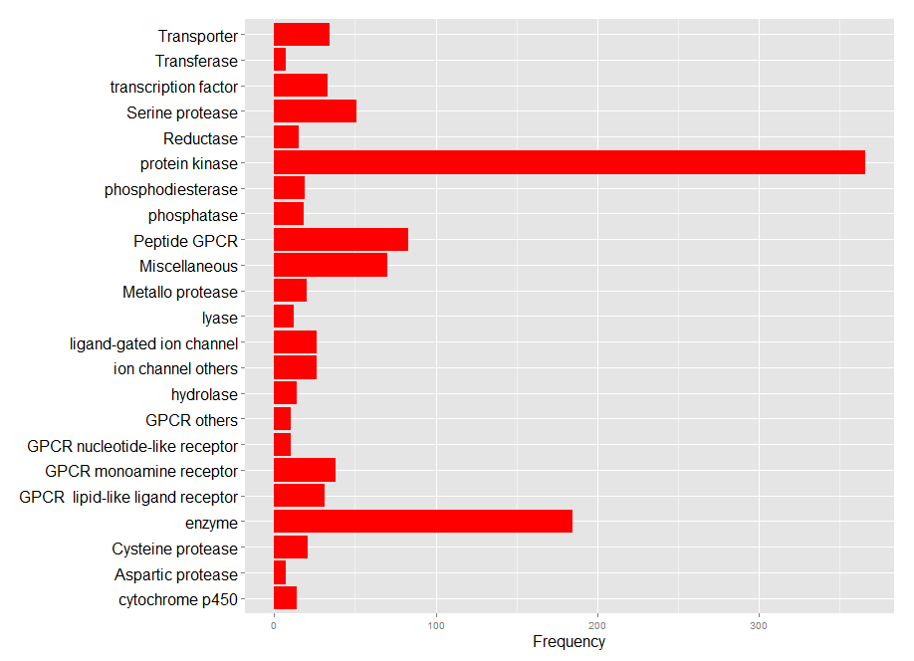
\includegraphics[width=0.75\columnwidth]{pfamily}
\end{figure}
}
\section{Result}
\subsection{Feature Selection}
\frame{
\frametitle{Feature Selection}
The protein family of Peptide GPCR including 85 proteins as examples.
\begin{itemize}
  \item
  Based on the definitions of chemical fingerprints, SUB1-SUB115, SUB264-SUB327 are removed.
  \item
  Chemical fingerprints with too low or high frequencies are removed.
  \item
  Non-parametric dynamic slicing method for marginal feature selection.
  \item
  284 features are finally kept.
\end{itemize}
}
%\subsection{Learning Pattern}
%\frame{
%%\frametitle{Learning Pattern}
%\begin{figure}
%  \centering
%  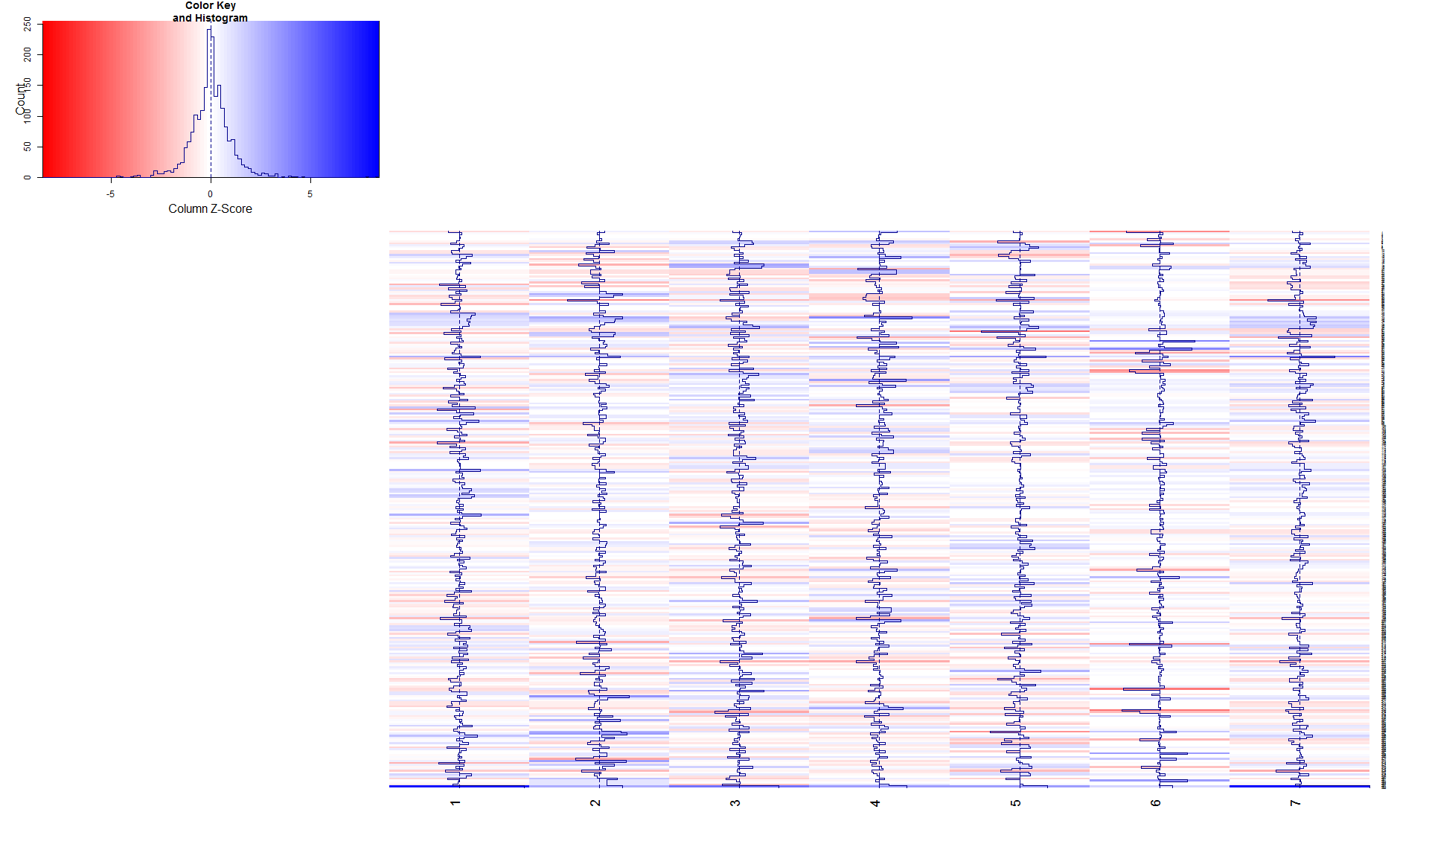
\includegraphics[width=1.1\columnwidth]{pattern}
%\end{figure}
%}
\subsection{Comparison with single-task model}
\frame{
\frametitle{Comparison with Ridge Regression}
\begin{figure}
  \centering
  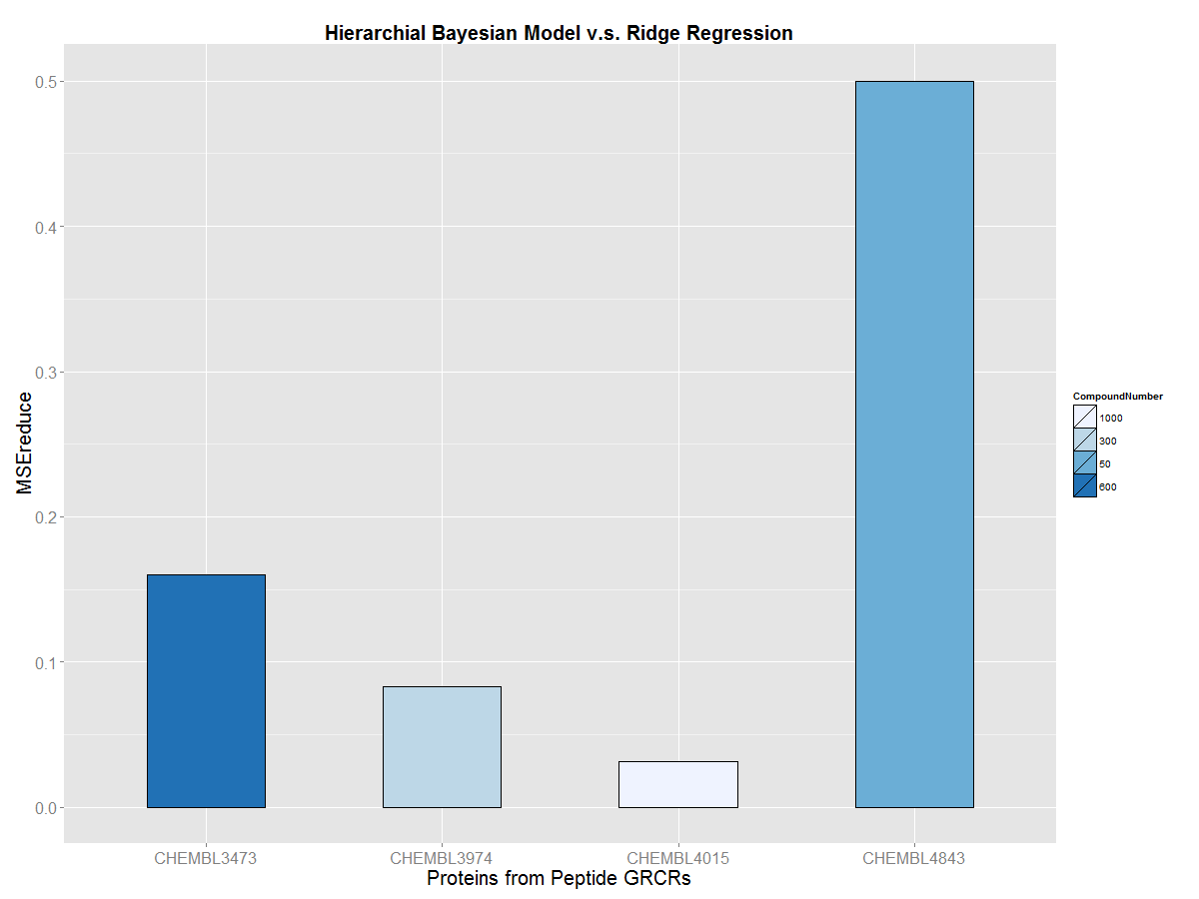
\includegraphics[width=0.9\columnwidth]{compare}
\end{figure}
}

\section{Discussion}
\frame{
\frametitle{Discussion}
\begin{itemize}
\item More compounds' fingerprints are being collected by the open-source chemoinformatics and machine learning package termed RDKit.
  %\item
  %A hierarchial Bayesian model is constructed to predict CPIs following the multi-task approach.
  %\item
  %More computational tests
  %\item
  %The relationship between proteins' pharmacological and genomic information
  \item
  Computational issue:
  \begin{itemize}
    \item
    High dimension v.s. Sparsity \\
    Colinearity
    \item
    Linear v.s. Nonlinear
  \end{itemize}
\end{itemize}
}
\end{document}